%%%%%%%%%%%%%%%%%%%%%%% file template.tex %%%%%%%%%%%%%%%%%%%%%%%%%
%
% This is a general template file for the LaTeX package SVJour3
% for Springer journals.          Springer Heidelberg 2010/09/16
%
% Copy it to a new file with a new name and use it as the basis
% for your article. Delete % signs as needed.
%
% This template includes a few options for different layouts and
% content for various journals. Please consult a previous issue of
% your journal as needed.
%
%%%%%%%%%%%%%%%%%%%%%%%%%%%%%%%%%%%%%%%%%%%%%%%%%%%%%%%%%%%%%%%%%%%
%
% First comes an example EPS file -- just ignore it and
% proceed on the \documentclass line
% your LaTeX will extract the file if required
\begin{filecontents*}{example.eps}
%!PS-Adobe-3.0 EPSF-3.0
%%BoundingBox: 19 19 221 221
%%CreationDate: Mon Sep 29 1997
%%Creator: programmed by hand (JK)
%%EndComments
gsave
newpath
  20 20 moveto
  20 220 lineto
  220 220 lineto
  220 20 lineto
closepath
2 setlinewidth
gsave
  .4 setgray fill
grestore
stroke
grestore
\end{filecontents*}
%
\RequirePackage{fix-cm}
%
%\documentclass{svjour3}                     % onecolumn (standard format)
%\documentclass[smallcondensed]{svjour3}     % onecolumn (ditto)
\documentclass[smallextended]{svjour3}       % onecolumn (second format)
%\documentclass[twocolumn]{svjour3}          % twocolumn
%
\smartqed  % flush right qed marks, e.g. at end of proof
%
\usepackage{graphicx}
\usepackage{amsmath}              
  {
      \newtheorem{assumption}{Assumption}
  }
\usepackage{amssymb}
\usepackage{graphicx}
%
% \usepackage{mathptmx}      % use Times fonts if available on your TeX system
%
% insert here the call for the packages your document requires
%\usepackage{latexsym}
% etc.
%
% please place your own definitions here and don't use \def but
% \newcommand{}{}
%
% Insert the name of "your journal" with
% \journalname{myjournal}
%
\begin{document}

\title{Quasi-structure in the dual Hessian for distributed MPC with non-delayed couplings%\thanks{Grants or other notes
%about the article that should go on the front page should be
%placed here. General acknowledgments should be placed at the end of the article.}
}
%\subtitle{Do you have a subtitle?\\ If so, write it here}

%\titlerunning{Short form of title}        % if too long for running head

\author{Emil Klintberg         \and
        Sebastien Gros %etc.
}

%\authorrunning{Short form of author list} % if too long for running head

\institute{Emil Klintberg \at
              first address \\
              Tel.: +123-45-678910\\
              Fax: +123-45-678910\\
              \email{fauthor@example.com}           %  \\
%             \emph{Present address:} of F. Author  %  if needed
           \and
           Sebastien Gros \at
              second address
}

\date{Received: date / Accepted: date}
% The correct dates will be entered by the editor


\maketitle

\begin{abstract}
Bla bla bla
\keywords{First keyword \and Second keyword \and More}
% \PACS{PACS code1 \and PACS code2 \and more}
% \subclass{MSC code1 \and MSC code2 \and more}
\end{abstract}

\section{Introduction}
Bla bla bla

\subsection{Motivation: Distributed MPC with non-delayed couplings}
We consider $M$ discrete time linear systems given by:
\begin{subequations}
\begin{align}
x_{1,i+1} & = A_{1,i} x_{1,i} + B_{1,i} u_{1,i} \\
& \vdots \\
x_{M,i+1} & = A_{M,i} x_{M,i} + B_{M,i} u_{M,i} 
\end{align}
\end{subequations}
where $x_{k,i} \in \mathbb{R}^{p_{k}}$ and $u_{k,i} \in \mathbb{R}^{m_{k}}$ represents the state and input of system $k$. We also assume state and input constraints:
\begin{subequations}
\begin{align}
x_{k,i} \in X_{k,i} \subseteq \mathbb{R}^{p_{k}} \\
u_{k,i} \in U_{k,i} \subseteq \mathbb{R}^{m_{k}}
\end{align}
\end{subequations}
Moreover, we assume non-delayed couplings between the systems:
\begin{equation}
h_i(x_{1,i}, u_{1,i}, \dots, x_{M,i}, u_{M,i}) = 0, \quad i = 0,\dots,N-1
\end{equation}
This means that we can state the MPC problem over the horizon $N$ as:
\begin{subequations}
\begin{align}
\min_{x_{k,i}, u_{k,i}} & \quad \sum_{k=1}^{M} \left( \sum_{i=0}^{N-1} \mathnormal{l}(x_{k,i}, u_{k,i}) + \mathnormal{l}_f(x_{k,N}) \right) \label{e:MPCobjective} \\
\text{s.t.} & \quad x_{k+1,i} = A_{k,i}x_{k,i} + B_{k,i}u_{k,i} \\
& \quad h_k(x_{k,1}, u_{k,1}, \dots, x_{k,M}, u_{k,M}) = 0 \label{e:MPCcouplings} \\
& \quad x_{k,i} \in X_{k,i}, \quad u_{k,i} \in U_{k,i} \label{e:MPCconstrains}
\end{align}
\end{subequations}

Furthermore, let us assume that the non-delayed couplings (\ref{e:MPCcouplings}) are linear, constraints (\ref{e:MPCconstrains}) are polyhedral and that the objective function (\ref{e:MPCobjective}) is quadratic, and introduce the following notation: $z_{k,i} = [x_{k,i}^T \quad u_{k,i}^T]^T \in \mathbb{R}^{n_{k}}$. The MPC problem can then be stated as:
\begin{subequations}
\label{e:problem}
\begin{align}
\min_z & \quad \sum_{k=1}^{M} \sum_{i=0}^N \frac{1}{2}z_{k,i}^TH_{k,i}z_{k,i} + c_{k,i}^Tz_{k,i} \label{e:1} \\
\text{s.t.} & \quad \sum_{k=1}^{M} F_{k,i}z_{k,i} = e_i \label{e:CoupConstControl} \\
& C_{k,i}z_{k,i} + D_{k,i+1}z_{k,i+1} = d_{k,i}  \label{e:dynamics} \\
& G_{k,i}z_{k,i} \leq f_{k,i}
\end{align}
\end{subequations}
where $H_{k,i} \in \mathbb{S}_{++}^{n_{k} \times n_{k}}$, $C_{k,i} \in \mathbb{R}^{l_{k} \times n_{k}}$, $D_{k,i+1} \in \mathbb{R}^{l_{k} \times n_{k}}$ and $d_{k,i} \in \mathbb{R}^{l_{k}}$ form the dynamics, $F_{k,i} \in \mathbb{R}^{r_{i} \times n_{k}}$ and $e_i \in \mathbb{R}^{r_i}$ yield the coupling constraints, $G_{k,i} \in \mathbb{R}^{t_{k} \times n_{k}}$ and $f_{k,i} \in \mathbb{R}^{t_{k}}$ form the local constraints.

Additionaly, to avoid an unnecessary heavy notation at places where we are only dealing with decomposition in space, we introduce the following augmented notations: $z_k = [z_{k,0}^T \dots, z_{k,N-1}^T]^T \in \mathbb{R}^{n_k}$. The MPC problem (\ref{e:problem}) can then be expressed as:
\begin{subequations}
\label{e:problem1}
\begin{align}
\min_z & \quad \sum_{k=1}^{M} \frac{1}{2}z_k^TH_k z_k + c_k^Tz_k \label{e:1} \\
\text{s.t.} & \quad \sum_{k=1}^{M} F_k z_k = e \label{e:CoupConst} \\
& C_k z_k = d_k \label{e:3} \\
& G_k z_k \leq f_k \label{e:ineqConst}
\end{align}
\end{subequations}
where $H_{k} \in \mathbb{S}_{++}^{(N+1)n_{k} \times (N+1)n_{k}}$, $C_{k} \in \mathbb{R}^{N l_{k} \times (N+1)n_{k}}$ and $d_{k} \in \mathbb{R}^{N l_{k}}$, $F_{k} \in \mathbb{R}^{(N+1) r \times (N+1) n_{k}}$ and $e \in \mathbb{R}^{(N+1)r}$, $G_{k} \in \mathbb{R}^{(N+1) t_{k} \times (N+1) n_{k}}$ and $f_{k} \in \mathbb{R}^{(N+1) t_{k}}$ and the matrices are accordingly given by:
\begin{subequations}
\begin{align*}
& H_k = \left[ \begin{array}{ccc}
H_{k,0} & & \\
 & \ddots & \\
 & & H_{k,N}
\end{array} \right], \\
& C_k = \left[ \begin{array}{ccccc} 
C_{k,0} & D_{k,1} &  &   &  \\
 & C_{k,1} & D_{k,2} &  &  \\
 &  & \ddots & \ddots &  \\
 &  &  & C_{k,N-1} & D_{k,N}
\end{array} \right], \\
& A_k = \left[ \begin{array}{ccc}
A_{k,0} & & \\
 & \ddots & \\
 & & A_{k,N}
\end{array} \right].
\end{align*}
\end{subequations}

\section{Prelimenaries}

%We consider a strictly convex QP of the form
%\begin{subequations}
%\label{e:problem1}
%\begin{align}
%\min_x & \quad \sum_{k=1}^{M} \frac{1}{2}x_k^TH_kx_k + c_k^Tx_x \label{e:1} \\
%\text{s.t.} & \quad \sum_{k=1}^{M} F_kx_k = e \label{e:CoupConst} \\
%& \quad x_k \in \mathcal{X}_k \label{e:3} 
%\end{align}
%\end{subequations}
%where, for all $k \in \{1,\dots,M \}$, $x_k \in \mathbb{R}^{n_k}$ are the decision variables with $x = [ x_1^T,\dots,x_M^T]^T \in \mathbb{R}^n$. Moreover, $H_k \in \mathbb{R}^{n_k \times n_k}$ are positive definite, i.e. for all $k \in \{ 1, \ldots, M \}$, $H_k \succ 0$, the sets $\mathcal{X}_k = \{ x_k \in \mathbb{R}^{n_k} | C_kx_k = d_k, A_kx_k \leq b_k \}$ are polyhedral, $C_k \in \mathbb{R}^{l_k \times n_k}$, $A_k \in \mathbb{R}^{m_k \times n_k}$, $F_k \in \mathbb{R}^{p \times n_k}$ and $e \in \mathbb{R}^p$ yield the coupling constraints.

\subsection{Dual decomposition with second-order information}

We introduce the dual variables $\lambda \in \mathbb{R}^{(N+1) r}$ corresponding to the coupling constraints (\ref{e:CoupConst}) and define the Lagrange function as
\begin{equation}
\mathcal{L}(z,\lambda) =  \sum_{k=1}^{M} ( \frac{1}{2}z_k^TH_kz_k + c_k^Tz_k ) + \lambda^T ( \sum_{k=1}^{M} F_k z_k - e )
\end{equation}
Note that $\mathcal{L}(z,\lambda)$ is separable in $z$, i.e.
\begin{equation}
\mathcal{L}(z,\lambda) = \sum_{k=1}^{M} \mathcal{L}_k (z_k,\lambda)
\end{equation}
with
\begin{equation}
\mathcal{L}_k(z_k,\lambda) = \frac{1}{2}z_k^TH_k z_k + c_k^T z_k + \lambda^T(C_k z_k - \frac{1}{M}d)
\end{equation}
The dual function $d(\lambda) = -\min_{z \in \mathcal{Z}} \mathcal{L}(z,\lambda)$ can thus be evaluated in parallel as:
\begin{equation}
\label{e:dualfunction}
d(\lambda) = -\sum_{k=1}^M \min_{z_k \in \mathcal{Z}_k} \mathcal{L}_k(z_k,\lambda)
\end{equation}

Since (\ref{e:problem1}) is strictly convex, (\ref{e:dualfunction}) is convex and continuously differentiable, but not twice differentiable. However, the Hessian of $d(\lambda)$ is a piecewise constant matrix and change with the active-set \cite{Kozma2014a}.

The non-smoothness implies that $d(\lambda)$ is not self-concordant and the solution to the dual problem is hence not easily tracked with Newton's method. However, if we relax the inequality constraints (\ref{e:ineqConst}) with a self-concordant log-barrier, according to:
\begin{subequations}
\label{e:relaxedproblem}
\begin{align}
\min_z & \quad \sum_{k=1}^{M} \frac{1}{2}z_k^TH_k z_k + c_k^T z_k - \tau \sum_{i=1}^{(N+1)t_k} \log([s_k]_i) \label{e:1} \\
\text{s.t.} & \quad \sum_{k=1}^{M} F_k z_k = e \\
& \quad C_k z_k = d_k \\
& \quad G_k z_k + s_k = f_k
\end{align}
\end{subequations}
where $\tau > 0$ will be referred to as the \emph{barrier parameter}, the resulting \emph{relaxed dual function} $d(\lambda, \tau)$ is self-concordant \cite{Necoara2009a}. This opens for the possibility of solving a sequence of dual problems $\left\{\min_\lambda d(\lambda, \tau) \right\}_{\tau \rightarrow 0}$ where each problem is self-concordant and therefore easily solved with Newton's method.

The relaxed dual function is separable and can be evaluated in parallel as
\begin{equation}
\label{e:relaxeddualfunction}
d(\lambda, \tau) = -\sum_{k=1}^N \min_{z_k \in \mathcal{Z}_k} \left( \mathcal{L}_k(z_k, \lambda) - \tau \sum_{i=1}^{m_k} \log([s_k]_i) \right)
\end{equation}

Hence, evaluating (\ref{e:relaxeddualfunction}) involves solving local subproblems of the form
\begin{equation}
\label{e:localproblem}
\begin{aligned}
\min_{z_k} & \quad \frac{1}{2}z_k^T H_k z_k + c_k^T z_k + \lambda^TF_k z_k - \tau \sum_{i=1}^{m_k} \log([s_k]_i) \\
\text{s.t.} & \quad C_k z_k = d_k \\ 
& \quad G_k z_k + s_k = f_k \\
& \quad s_k \geq 0
\end{aligned}
\end{equation}


The relaxed dual problem then reads
\begin{equation}
\min_{\lambda} d(\lambda, \tau)
\end{equation}
from which solution, the solution to (\ref{e:relaxedproblem}) can be recovered according to strong duality \cite{Boyd2004}.

Strict convexity also implies that the gradient of $d(\lambda, \tau)$ is given by the residual of the coupling constraints \cite{Bertsekas1989}, i.e.
\begin{equation}
\label{e:dualgradient}
\nabla d(\lambda, \tau) = -\sum_{k=1}^N F_k z_k^*(\lambda, \tau) + e
\end{equation}
where $z_k^*(\lambda, \tau) = \arg \min_{z_k \in \mathcal{Z}_k} \mathcal{L}_k(z_k, s_k, \lambda, \tau)$.
The dual Hessian is then given by
\begin{equation}
\label{e:dualhessian}
\nabla^2 d(\lambda, \tau) = -\sum_{k=1}^N F_k \frac{\partial z_k^*(\lambda, \tau)}{\partial \lambda}
\end{equation}

A Newton direction $\Delta \lambda$ in the dual space can then be obtained as a solution to the Newton system
\begin{equation}
\label{e:NewtonSystem}
\nabla^2 d(\lambda, \tau) \Delta \lambda + \nabla d(\lambda, \tau) = 0
\end{equation}

\section{Structure in the dual Hessian}

\subsection{Dual Hessian}

By introducing $y_k = \tau/s_k \in \mathbb{R}^{m_k}$, the KKT conditions to (\ref{e:localproblem}) are given by
\begin{subequations}
\label{e:KKTconditions}
\begin{align}
& r_k(w_k^*, \lambda, \tau) = \left[ \begin{array}{c}
r_{Dk}(w_k^*, \lambda) \\
r_{Ek}(w_k^*) \\
r_{Ik}(w_k^*) \\
r_{Ck}(w_k^*, \tau)
\end{array} \right] = 0 \\
& s_k^* > 0, \quad y_k^* > 0
\end{align}
\end{subequations}
where we use the notation $w_k = [z_k^T, \mu_k^T, y_k^T, s_k^T ]^T$ for the local primal-dual variables and $r_k(w_k, \lambda, \tau)$ is given by:
\begin{subequations}
\begin{align}
& r_{D_k}(w_k, \lambda) = H_k z_k + c_k + F_k^T \lambda + C_k^T \mu_k + G_k^T y_k \\
& r_{Ek}(w_k) = C_k z_k - d_k \\
& r_{Ik}(w_k) = G_k z_k + s_k - f_k \\
& r_{Ck}(w_k, \tau) = Y_k s_k - \tau \mathbf{1} 
\end{align}
\end{subequations}

As we have seen in previous section, in order to form the dual Hessian we need to compute $\frac{\partial z_k^*}{\partial \lambda}$, where $z_k^* = z_k^*(\lambda)$ is the optimal primal solution and is hence fulfilling (\ref{e:KKTconditions}). By differentiating (\ref{e:KKTconditions}), the following linear system is obtained:
\begin{equation}
\label{e:SensitivityLambda}
\left[ \begin{array}{cccc}
H_k & C_k^T & G_k^T & 0 \\
C_k & 0 & 0 & 0 \\
G_k & 0 & 0 & I \\
0 & 0 & S_k & Y_k
\end{array} \right]
\left[ \begin{array}{c}
\frac{\partial z_k^*}{\partial \lambda} \\
\frac{\partial \mu_k^*}{\partial \lambda} \\
\frac{\partial y_k^*}{\partial \lambda} \\
\frac{\partial s_k^*}{\partial \lambda}
\end{array} \right] = -
\left[ \begin{array}{c}
F_k^T \\
0 \\
0 \\
0
\end{array} \right]
\end{equation}

If block elimination of (\ref{e:SensitivityLambda}) is used, the \emph{normal equations} can be formed \cite{Wright1997},
\begin{subequations}
\begin{align}
& \Lambda_k \frac{\partial \mu_k^*}{\partial \lambda} = -C_k \Phi_k^{-1} F_k^T \label{e:firstNormalEquation} \\
& \Phi_k \frac{\partial z_k^*}{\partial \lambda} = -F_k^T - C_k^T \frac{\partial \mu_k^*}{\partial \lambda} \label{e:secondNormalEquation} \\
& \frac{\partial s_k^*}{\partial \lambda} = -G_k \frac{\partial z_k^*}{\partial \lambda} \\
& \frac{\partial y_k^*}{\partial \lambda} = -S^{-1} Y \frac{\partial s_k^*}{\partial \lambda}
\end{align}
\end{subequations}
where $\Phi_k = H_k + G_k^T S_k^{-1} Y_k G_k \in \mathbb{S}_{++}^{(N+1)n_k \times (N+1)n_k}$ and $\Lambda_k = C_k \Phi_k^{-1} C_k^{T} \in \mathbb{S}_{++}^{N l_k \times N l_k}$. By using (\ref{e:firstNormalEquation}) and (\ref{e:secondNormalEquation}), it can be obtained that
\begin{equation}
\label{e:localcontributions}
F_k \frac{\partial z_k}{\partial \lambda} = -F_k (\Phi_k^{-1} - \Phi_k^{-1} C_k^T \Lambda_k^{-1} C_k \Phi_k^{-1}) F_k^T
\end{equation}
This means that the dual Hessian (\ref{e:dualhessian}) can be written as
\begin{equation}
\label{e:dualhessian2}
\nabla^2 d(\lambda, \tau) = \sum_{k=1}^M F_k (\Phi_k^{-1} - \Phi_k^{-1} C_k^T \Lambda_k^{-1} C_k \Phi_k^{-1}) F_k^T
\end{equation}

Let us now turn our attention to the structure coming from the time domain. We have already seen that $C_k$ is block bidiagonal, and it can trivially be realized that $\Phi_k$ is block diagonal. This means that $\Lambda_k$ has a block tridiagonal structure given by:
\begin{equation}
\Lambda_k = \left[ \begin{array}{cccc} 
\Lambda_{11} &  \Lambda_{12} &   &  \\
\Lambda_{12}^T &  \Lambda_{22} & \ddots  &  \\
  &  \ddots & \ddots  & \Lambda_{N-1,N} \\
    &   & \Lambda_{N-1,N}^T  & \Lambda_{N,N} \\
\end{array} \right] \in \mathbb{S}_{++}^{N l_{k} \times N l_{k}}
\end{equation}
where
\begin{subequations}
\label{e:LambdaComponents}
\begin{align}
& \Lambda_{i,i} = C_{k,i-1}\Phi_{k,i-1}^{-1}C_{k,i-1}^T + D_{k,i}\Phi_{k,i}^{-1}D_{k,i}^T \in \mathbb{R}^{l_{k,} \times l_{k}} \\
& \Lambda_{i,i+1} = D_{k,i} \Phi_{k,i}^{-1}C_{k,i}^T \in \mathbb{R}^{l_{k} \times l_{k}}
\end{align}
\end{subequations}

Accordingly, all matrices in (\ref{e:dualhessian2}) are banded except $\Lambda_k^{-1}$ which in general is dense.

\subsection{Decaying of the dual Hessian} \label{S:TheoreticalDecay}
Let us first assume that the problem data is bounded. In other words, let us assume the following:
\begin{assumption} \label{a:BoundedData}
The row and column absolute sums of Jacobians of equality constraints (i.e. (\ref{e:CoupConst}) and (\ref{e:3})) are bounded. Hence:
\begin{enumerate}
\item $\| C_{k,i} \|_\infty \leq \gamma$ and $\| C_{k,i} \|_1 \leq \gamma$
\item $\| D_{k,i} \|_\infty \leq \gamma$ and $\| D_{k,i} \|_1 \leq \gamma$
\item $\| F_{k,i} \|_\infty \leq \gamma$ and $\| F_{k,i} \|_1 \leq \gamma$
\end{enumerate}
\end{assumption}
It should be observed that Assumption \ref{a:BoundedData} is not by any means restrictive, since any solver would struggle with a problem where it is not fulfilled. 

Furthermore, we assume boundedness of $\Phi_k^{-1}$:
\begin{assumption} \label{a:BoundedConditioning}
The row and column absolute sums of $\Phi_k^{-1}$ are bounded. Hence:
\begin{equation}
\| \Phi_{k,i}^{-1} \|_\infty = \| \Phi_{k,i}^{-1} \|_1 \leq \gamma_{\Phi_k^{-1}}, \quad \forall i
\end{equation}
\end{assumption}
Possible problems with interior-point methods are related to numerical difficulties due to ill-conditioning \cite{}. This might occur since elements in $S_k^{-1}Y_k$ can be close to zero in late iterations when $\tau$ is small. Our experience is however that this is not a major issue in practice, which is also supported by commercial interior-point implementations \cite{}. Moreover, since we assume that (\ref{e:problem}) is strongly convex, the eigenvalues of $\Phi_k$ are lower bounded by the smallest eigenvalue of $H_k$, even when $S_k^{-1}Y_k$ is singular. According to this reasoning it is not restrictive to assume boundedness of $\Phi_k^{-1}$.

Inverses of sparse matrices are in general dense, but individual elements are often small in absolute value. Since $\Lambda_k$ is banded, symmetric and positive definite, we will relay our analysis on the following classical result:

\begin{lemma} \label{l:decay}
If $A$ is Hermitian positive definite and $m$-banded ($[A]_{ij} = 0$ if $|i-j| > m$), the entries of $A^{-1}$ satisfy the following bound:
\begin{equation}
|[A^{-1}]_{ij}| < K\omega^{|i-j|}, \quad \forall i,j
\end{equation}
where $[a,b]$ is the smallest interval containing the spectrum $\sigma(A)$ of $A$, $K = \max \{ a^{-1}, K_0 \}$, $K_0 = (1 + \sqrt{\kappa})$, $\omega = q^{1/m}$, $q = \frac{\sqrt{\kappa} - 1}{\sqrt{\kappa} + 1}$, $\kappa = \frac{b}{a}$.
\end{lemma}
\begin{proof}
A proof is given in \cite{}. \qed
\end{proof}

This means that the entries of $A^{-1}$ are bounded by an exponentially decaying function along each row or column. However, the bound depends on the condition number and the bandwidth of the matrix. Matrices with a high condition number and/or a high bandwidth can accordingly result in a large $K$ and $\omega \approx 1$, leading to a slow decay. The opposite, i.e. a low condition number and a small band, would result in a rapid decay.

Observe that due to the block tridiagonal structure of $\Lambda_k$, it is $3 l_k$-banded. Moreover, if we introduce the notation
\begin{equation}
\Lambda_k^{-1} = \left[ \begin{array}{cccc}
T_{11} & T_{21}^T & \hdots & T_{N+1,1}^T \\
T_{21} & T_{22} & \hdots & T_{N+1,2}^T \\
\vdots & \vdots  & \ddots & \vdots \\
T_{N+1,1} & T_{N+1,2} & \hdots & T_{N+1,N+1}
\end{array} \right]
\end{equation}
where $T_{i,j} \in \mathbb{R}^{l_{k} \times l_{k}}$, we can establish the following proposition:

\begin{proposition} \label{p:decayofLambda}
The off-diagonal blocks (i.e. $T_{i,j}$ where $i - j > 0$) in $\Lambda_k^{-1}$ satisfy the following bounds:
\begin{subequations} \label{e:decayofLambda}
\begin{align}
\| T_{i,j} \|_\bullet \leq K_{\Lambda_k} \omega_{\Lambda_k}^{i - j} \\
\end{align}
\end{subequations}
where $\bullet$ represents $\infty$ and $1$, $\sigma_{\min}(\Lambda_k)$ and $\kappa_{\Lambda_k}$ are the the smallest singular value and the condition number of $\Lambda_k$ respectively, $K_{\Lambda_k} = \max \{ \sigma_{\min}(\Lambda_k)^{-1}, 1 + \sqrt{\kappa_{\Lambda_k}} \} l_k \omega_{\Lambda_k}^{1/l_k}$ and $\omega_{\Lambda_k} = \left( \frac{\sqrt{\kappa_{\Lambda_k}} - 1}{\sqrt{\kappa_{\Lambda_k}} + 1} \right)^{\frac{1}{3}}$.
\end{proposition}

\begin{proof}
According to Lemma \ref{l:decay}, the element in $T_{i,j}$ with the largest bound is located in the top-right corner, and is hence element $[\Lambda_k^{-1}]_{i l_k + 1, j l_k}$. By directly applying Lemma \ref{l:decay} it follows that:
\begin{equation}
\max \left| [ T_{ij} ] \right| \leq \max \{ \sigma_{min}(\Lambda_k)^{-1}, 1 +  \sqrt{\kappa_{\Lambda_k}} \} \left( \frac{ \sqrt{\kappa_{\Lambda_k}} - 1}{ \sqrt{\kappa_{\Lambda_k}} + 1} \right)^{\frac{1}{3l_k}((i - j)l_k + 1)}
\end{equation}
where $\max \left| [ T_{ij} ] \right| $ refers to the maximum absolute value of the components in $T_{ij}$. Moreover, since there are $l_k$ elements in each row or column of a block $T_{i,j}$, we obtain the bounds given in (\ref{e:decayofLambda}).
\qed
\end{proof}

The constants $K_{\Lambda_k}$ and $\omega_{\Lambda_k}$ in Proposition \ref{p:decayofLambda} depends heavily on the conditioning of $\Lambda_k$, which indeed for interior point methods in general can be very high for small values of $\tau$. It should however be understood that strong convexity of (\ref{e:problem}), should improve the worst case conditioning of $\Phi_k$ and hence also of $\Lambda_k$.

To gain some perspective, we have concluded that $\Lambda_k^{-1}$ is decaying exponentially towards the off-diagonal corners and that all other matrices in (\ref{e:dualhessian2}) are banded. This suggests that also $\nabla_{\lambda \lambda}^2 d(\lambda, \tau)$ should decay towards the off-diagonal corners. To maintain a simple reasoning, one more stepping stone will be used before arriving at the main results of this section. Therefore, let us introduce the notation:
\begin{equation}
C_k^T \Lambda_k^{-1} C_k = \left[ \begin{array}{cccc}
V_{11} & V_{21}^T & \hdots & V_{N+1,1}^T \\
V_{21} & V_{22} & \hdots & V_{N+1,2}^T \\
\vdots & \vdots  & \ddots & \vdots \\
V_{N+1,1} & V_{N+1,2} & \hdots & V_{N+1,N+1}
\end{array} \right]
\end{equation}
where $V_{ij} \in \mathbb{R}^{l_{k} \times l_{k}}$, and look at the decay of $C_k^T \Lambda_k^{-1} C_k$.

\begin{proposition}
The off diagonal blocks (i.e. $V_{i,j}$ where $i - j > 0$) of $C_k^T \Lambda_k^{-1} C_k$ satisfy the following bounds:
\begin{subequations}
\begin{align}
\| V_{i,j} \|_\bullet \leq \gamma^2 \bar{K}_{\Lambda_k} \omega_{\Lambda_k}^{i-j} \\
\end{align}
\end{subequations}
where $\bar{K}_{\Lambda_k} = (2 + \omega_{\Lambda_k} + \omega_{\Lambda_k}^{-1}) \omega_{\Lambda_k}^{-1} K_{\Lambda_k}$ and $\bullet$ represents $\infty$ and $1$.
\end{proposition}
\begin{proof}
Bla bla bla
\qed
\end{proof}

%\begin{proposition}
%Let 
%\begin{equation}
%\gamma_{ij} = \max_{i-1 \leq t \leq i, j-1 \leq r \leq j} | \alpha_t - \beta_r |
%\end{equation}
%Then the following bounds hold:
%\begin{subequations}
%\begin{align}
%& \| V_{i,j} \|_\infty \leq \theta_{ij} K \lambda^{\gamma_{ij}} \\
%& \| V_{i,j} \|_1 \leq \psi_{ij} K \lambda^{\gamma_{ij}}
%\end{align}
%\end{subequations}
%where
%\begin{subequations}
%\begin{align}
%& \theta_{ij} = \| D_{i-1}^T \|_\infty \| D_{j-1} \|_\infty + \| C_{i-1}^T \|_\infty \| D_{j-1} \|_\infty + \| D_{i-1}^T \|_\infty \| C_{j-1} \|_\infty + \| C_{i-1}^T \|_\infty \| C_{j-1} \|_\infty \\
%& \psi_{ij} = \| D_{i-1}^T \|_1 \| D_{j-1} \|_1 + \| C_{i-1}^T \|_1 \| D_{j-1} \|_1 + \| D_{i-1}^T \|_1 \| C_{j-1} \|_1 + \| C_{i-1}^T \|_1 \| C_{j-1} \|_1 
%\end{align}
%\end{subequations}
%\end{proposition}
%\begin{proof}
%By realizing that
%\begin{equation} 
%V_{ij} = D_{i-1}^T T_{i-1,j-1} D_{j-1} + C_{i-1}^T T_{i,j-1} D_{j-1} + D_{i-1}^T T_{i-1,j} C_{j-1} + C_{i-1}^T T_{i,j} C_{j-1}
%\end{equation}
%the bounds trivially follows by using Proposition X, Cauchy-Schwarz inequality and that
%\begin{equation}
%\lambda^{\gamma_{ij}} \geq \lambda^{| \alpha_i - \beta_j |}
%\end{equation}
%\qed
%\end{proof}

Let us now introduce the notation:
\begin{equation}
\nabla^2 d(\lambda, \tau) = \left[ \begin{array}{cccc}
W_{11} & W_{21}^T & \hdots & W_{N+1,1}^T \\
W_{21} & W_{22} & \hdots & W_{N+1,2}^T \\
\vdots & \vdots  & \ddots & \vdots \\
W_{N+1,1} & W_{N+1,2} & \hdots & W_{N+1,N+1}
\end{array} \right]
\end{equation}
where $W_{i,j} \in \mathbb{R}^{r_i \times r_j}$. We can now establish a decay towards the off-diagonal corners of $\nabla^2 d(\lambda, \tau)$.

\begin{proposition} \label{p:DecayHessian}
The off-diagonal blocks (i.e. $W_{i,j}$ where $i - j > 0$) of $\nabla^2 d(\lambda, \tau)$ satisfy the following bounds:
\begin{subequations}
\begin{align}
\| W_{i,j} \|_\bullet \leq \sum_{k=1}^M \gamma^4 \gamma_{\Phi_k^{-1}}^2 \bar{K}_{\Lambda_k} \omega_{\Lambda_k}^{i-j} \\
\end{align}
\end{subequations}
where $\bullet$ represents $\infty$ and $1$.
\end{proposition}
\begin{proof}
To be done.
\end{proof}

Moreover, let us continue by finding a bound on the euclidean distance between $\nabla^2 d(\lambda, \tau)$ and a band along its diagonal. To do so, we start by recalling Gershgorin's circle theorem:
\begin{theorem} \label{l:Gerschgorin}
For $A \in \mathbb{R}^{n \times n}$ with elements $a_{ij}$, let $R_i = \sum_{j \neq i} | a_{ij} |$ be the sum of the absolute values of the non-diagonal entries in the row $i$. Let $D(a_{ii},R_i)$ be the closed disc centered in $a_{ii}$ with radius $R_i$, then every eigenvalue of $A$ lies within at least one of the discs $D(a_{ii}, R_i)$.
\end{theorem}
\begin{proof}
A proof is given in \cite{}.
\qed
\end{proof}

Finally, we can establish our main result:
\begin{lemma} \label{l:EuclidianDistance}
Let $ \lfloor \nabla^2 d(\lambda, \tau) \rceil_{\mathcal{M}}$ represent the diagonal $\mathcal{M}$-block band of $\nabla^2 d(\lambda, \tau)$. The following bound holds:
\begin{equation} \label{e:EuclidianDistance}
\| \lfloor \nabla^2 d(\lambda, \tau) \rceil_{\mathcal{M}} - \nabla^2 d(\lambda, \tau) \|_2 \leq \left( N -\frac{\mathcal{M} - 1}{2} \right) \sum_{k=1}^M \gamma^4 \gamma_{\Phi_k^{-1}}^2 \tilde{K}_{\Lambda_k} \omega_{\Lambda_k}^{\frac{\mathcal{M} - 1}{2}}
\end{equation}
where $\tilde{K}_{\Lambda_k} = \bar{K}_{\Lambda_k} \omega_{\Lambda_k} =  (2 + \omega_{\Lambda_k} + \omega_{\Lambda_k}^{-1}) K_{\Lambda_k}$.
\end{lemma}
\begin{proof}
Since $\lfloor \nabla^2 d(\lambda, \tau) \rceil_{\mathcal{M}} - \nabla^2 d(\lambda, \tau)$ is symmetric, its singular values collapse into the absolute value of its eigenvalues. The problem of finding a bound on the $2$-norm is hence reduced to the problem of bounding the magnitude of the largest eigenvalue.

First, observe that all diagonal elements of $\lfloor \nabla^2 d(\lambda, \tau) \rceil_{\mathcal{M}} - \nabla^2 d(\lambda, \tau)$ are zero. This means that every Gershgorin disc will be centered in the origin, and a bound on the largest eigenvalue can be found by finding the largest radius of a Gershgorin disc.

The blocks $W_{i,j}$ in $\lfloor \nabla^2 d(\lambda, \tau) \rceil_{\mathcal{M}} - \nabla^2 d(\lambda, \tau)$ with the largest bound is located next to the diagonal band of zeros, i.e. where $i - j = \frac{\mathcal{M} - 1}{2} + 1$. Furthermore, there is at least $N -\frac{\mathcal{M} - 1}{2}$ nonzero blocks at each block row. Each block is upper bounded by Proposition X. This means that we can establish a bound on the radius of the Gershgorin discs, and hence the following:
\begin{equation}
\| \lfloor \nabla^2 d(\lambda, \tau) \rceil_{\mathcal{M}} - \nabla^2 d(\lambda, \tau) \|_2 \leq \left( N -\frac{\mathcal{M} - 1}{2} \right) \sum_{k=1}^M \gamma^4 \gamma_{\Phi_k^{-1}}^2 \bar{K}_{\Lambda_k} \omega_{\Lambda_k}^{\frac{\mathcal{M} - 1}{2} + 1}
\end{equation}
Equation (\ref{e:EuclidianDistance}) is then directly obtained by introducing $\tilde{K}_{\Lambda_k} = \bar{K}_{\Lambda_k} \omega_{\Lambda_k}$.
\qed
\end{proof}
Say something about the principal behavior of the bound...

It is well known that the use of an inexact Hessian will degrade the convergence of Newton's method to a linear rate \cite{}. However, let us still look at the relative error in the Newton direction that we get from using $\lfloor \nabla^2 d(\lambda, \tau) \rceil_{\mathcal{M}}$ instead of $\nabla^2 d(\lambda, \tau)$. First, recall the following lemma:
\begin{lemma} \label{l:InexactSolution}
If $x$ is a solution to $Ax = b$ and $\hat{x}$ is a solution to the pertubed system $(A + F) \hat{x} = b + f$, then the following bound holds:
\begin{equation}
\frac{\| \hat{x} - x \|_2}{\| x \|_2} \leq \kappa (A) (\rho_A - \rho_b)
\end{equation}
where $\kappa (A)$ represents the condition number of $A$, $\rho_A = \frac{\| F \|_2}{\| A \|_2}$ and $\rho_b = \frac{\| f \|_2}{\| b \|_2}$.
\end{lemma}
\begin{proof}
A proof is given in \cite{}.
\end{proof}

Accordingly, by combining Lemma \ref{l:EuclidianDistance} and Lemma \ref{l:InexactSolution} we can establish the following:
\begin{lemma}
If $\Delta \hat{\lambda}$ is a solution to $\lfloor \nabla^2 d(\lambda, \tau) \rceil_{\mathcal{M}} \Delta \hat{\lambda} = -\nabla d(\lambda,\tau)$, the following bound on the relative error compared to the true Newton direction $\Delta \lambda$ holds:
\begin{equation} \label{e:InexactSolution}
\frac{\| \Delta \hat{\lambda} - \Delta \lambda \|_2}{\| \Delta \lambda \|_2} \leq \| \nabla^2 d(\lambda,\tau)^{-1} \|_2 (N -\frac{\mathcal{M} - 1}{2}) \sum_{k=1}^M \gamma^4 \gamma_{\Phi_k^{-1}}^2 \tilde{K}_{\Lambda_k} \omega_{\Lambda_k}^{\frac{\mathcal{M} - 1}{2}}
\end{equation}
\end{lemma}
\begin{proof}
We can view $\Delta \hat{\lambda}$ as a solution to a perturbed system:
\begin{equation}
\left( \nabla^2 d(\lambda, \tau) + (\lfloor \nabla^2 d(\lambda, \tau) \rceil_{\mathcal{M}} - \nabla^2 d(\lambda, \tau)) \right) \Delta \hat{\lambda} = -\nabla d(\lambda, \tau)
\end{equation}
Equation (\ref{e:InexactSolution}) follows then directly from Lemma \ref{l:EuclidianDistance} and Lemma \ref{l:InexactSolution}.
\qed
\end{proof}

\section{Numerical experiments}

\subsection{Decaying of the dual Hessian}

\subsubsection{A small problem}

As an example of a small problem, we use a randomly generated problem with $4$ subproblems (i.e. $M=4$), where each subproblem has $N = 10$, $6$ states and $4$ controls and hence $n_k = 10$, and each time instance has $4$ coupling constraints.

\begin{figure}[h]
  \centering
  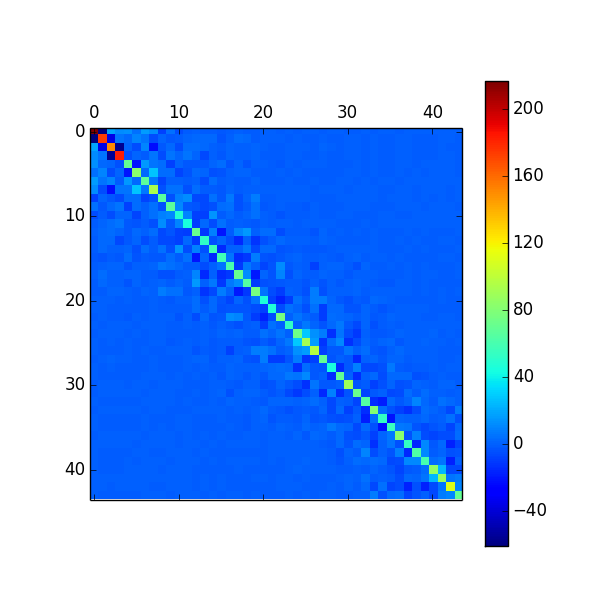
\includegraphics[scale = 0.5]{./Figures/SmallProblemLargeTau.png}\\
  \caption{$\tau = 1$}
  \label{f:SmallProblemLargeTau}
\end{figure}

According to Section \ref{S:TheoreticalDecay}, we expect a slower decay when the conditioning of $S_k^{-1}Y_k$ gets worse, i.e. when we reduce $\tau$. Surprisingly, this is something that does not seem to have a big influence in practice. To illustrate this, Figure \ref{f:SmallProblemSmallTau} shows the dual Hessian for the same problem as in Figure \ref{f:SmallProblemLargeTau}, but with $\tau=10^{-5}$.

\begin{figure}[h]
  \centering
  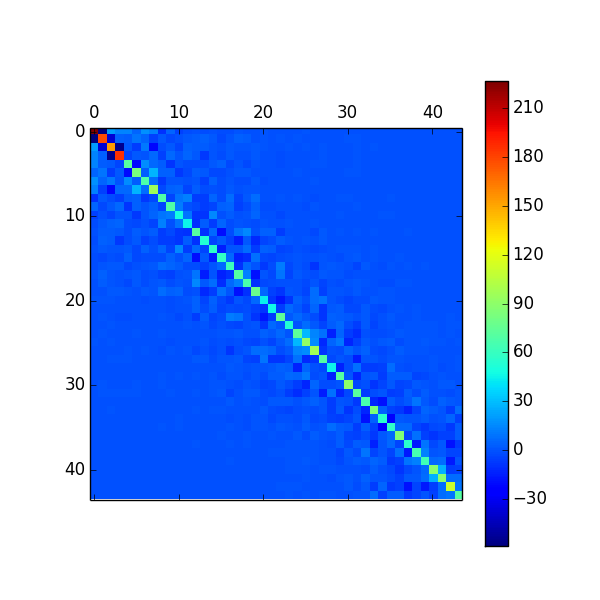
\includegraphics[scale = 0.5]{./Figures/SmallProblemSmallTau.png}\\
  \caption{$\tau = 10^{-5}$}
  \label{f:SmallProblemSmallTau}
\end{figure}

\subsubsection{A large problem}

\subsection{Newton steps with inexact Hessian}

%\begin{acknowledgements}
%If you'd like to thank anyone, place your comments here
%and remove the percent signs.
%\end{acknowledgements}

% BibTeX users please use one of
%\bibliographystyle{spbasic}      % basic style, author-year citations
\bibliographystyle{spmpsci}      % mathematics and physical sciences
%\bibliographystyle{spphys}       % APS-like style for physics
%\bibliography{}   % name your BibTeX data base

% Non-BibTeX users please use
\bibliography{optec}

\end{document}
% end of file template.tex

